% Only Optimization through Conclusion is revised; the protected prefix is unchanged.
\typeout{GLOBECOM_LAYOUT textheight=\the\textheight;columnwidth=\the\columnwidth;textwidth=\the\textwidth;topmargin=\the\topmargin;headheight=\the\headheight;headsep=\the\headsep;voffset=\the\voffset}
\raggedbottom
\section{Joint Source and Mobility Optimization}
\label{sec:optimization}
Cloud blockage favors spatial adaptation, but UAV motion incurs travel
cost. We jointly consider source selection, stationary deployment, and
mobility-aware positioning.
The finite catalog $\mathcal G=\{(\nu,V_A)\}$ contains 197 MB-shaped and
36 uniform 256-QAM ensembles. Source selection is
\begin{equation}
 \mathcal P_1:\quad K_j^\star=
 \left[\max_{(\nu,V_A)\in\mathcal G}K_j(\nu,V_A)\right]^+.
 \label{eq:p1}
\end{equation}
Each candidate uses its own exact source moments and fading noise.
Maximize raw rate before clipping; optimality is finite-catalog.
With $S_{j,n}=(1-c_{j,n})K_j^\star$, the best fixed position is
\begin{equation}
 \mathcal P_2:\quad j_{\rm fix}^\star=
 \arg\max_j\frac{1}{N_t}\sum_{n=1}^{N_t}S_{j,n}.
 \label{eq:p2}
\end{equation}
For a trajectory $j_n\in\{1,\ldots,J\}$, define
$d_{i,j}=\|\mathbf q_i-\mathbf q_j\|_2$. The mobility problem is
\begin{align}
 \mathcal P_3:\quad\max_{\{j_n\}}\quad&
 \frac{1}{N_t}\sum_{n=1}^{N_t}S_{j_n,n}
 -\frac{\lambda}{D_{\rm ref}}\sum_{n=2}^{N_t}d_{j_{n-1},j_n}
 \label{eq:p3}\\
 \mathrm{s.t.}\quad&d_{j_{n-1},j_n}\le v_{\max}\Delta t,
                  \quad n=2,\ldots,N_t.\nonumber
\end{align}
Here $U=\overline K-\lambda D/D_{\rm ref}$ balances mean usable rate
$\overline K$ and total distance $D$; $\lambda\ge0$ is in bit/use and
$D_{\rm ref}>0$ normalizes distance. Staying and free initial placement
are allowed, with no deployment or return cost. Distance is a cost
surrogate, not calibrated propulsion energy.

\section{Proposed Solution}
\label{sec:method}
P1 exhausts the catalog once per clear-sky position; P2 compares all $J$
mission means. Let $\mathcal N(j)=\{i:d_{i,j}\le v_{\max}\Delta t\}$,
including staying. Greedy starts at
$j_1^{\rm G}\in\arg\max_jS_{j,1}$ and then selects
\begin{equation}
 j_n^{\rm G}\in\arg\max_{j\in\mathcal N(j_{n-1}^{\rm G})}
 \left[S_{j,n}-\frac{N_t\lambda}{D_{\rm ref}}d_{j_{n-1}^{\rm G},j}\right].
 \label{eq:greedy}
\end{equation}
This $O(N_tJ)$ policy observes the current slot only. DP instead retains
the best prefix ending at each position:
\begin{align}
 F_1(j)&=S_{j,1},\label{eq:dp_init}\\
 F_n(j)&=S_{j,n}+\max_{i\in\mathcal N(j)}
 \left[F_{n-1}(i)-\frac{N_t\lambda}{D_{\rm ref}}d_{i,j}\right].
 \label{eq:dp}
\end{align}
Store maximizing predecessors, choose the best terminal state, and
backtrack. Then
$U^\star=\max_jF_{N_t}(j)/N_t$ in dense worst-case time $O(N_tJ^2)$,
with $O(N_tJ)$ backpointers and an $O(J^2)$ distance matrix.
P2 and DP know the complete cloud sequence offline. DP has no smaller
$U$ than P2 or Greedy, but need not dominate unpenalized rate or availability.
Its advantage also includes future information and initial-position selection.

\begin{figure*}[!t]
\centering
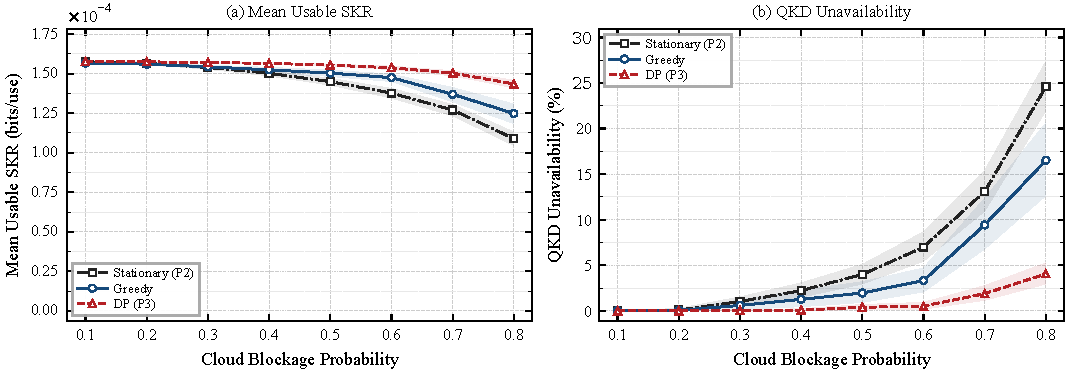
\includegraphics[width=\textwidth]{figures/fig2_cloud_blockage.pdf}
\caption{Cloud blockage sensitivity at $\lambda_{\rm ref}$: (a) mean usable
rate; (b) zero-rate unavailability. Stationary, Greedy, and DP share 100
paired missions; bands are pointwise 95\% whole-mission bootstrap intervals.}
\label{fig:cloud}
\end{figure*}

\section{Numerical Results and Discussion}
\label{sec:numerical}
Table~\ref{tab:parameters} gives the synthetic baseline; cell centers are
$50,150,\ldots,950$ m per axis. Gaussian-copula clouds use spatial covariance
$\exp(-d_{i,j}/\ell)$ and latent AR(1) coefficient $\rho$. Comparisons share
100 mission IDs (0--99); uncertainty uses saved whole-mission bootstrap
intervals. Availability means $S>0$, without an engineering threshold.
The presentation follows~\cite{gong2020}.

\begin{table}[!t]
\caption{Synthetic Baseline and Recorded Optical Parameters}
\label{tab:parameters}
\centering
\begin{tabular}{@{}ll@{}}
\toprule
Parameter & Value\\
\midrule
HAP / UAV altitude & 20 / 1 km\\
HAP horizontal position & $(11419.6551,450)$ m\\
Flight region / candidates & $1\times1$ km$^2$ / 100\\
Mission slots / slot duration & 30 / 20 s\\
$v_{\max}$ / $D_{\rm ref}$ & 15 m/s / 1000 m\\
Cloud $(p,\ell,\rho)$ & $(0.4,250\,\mathrm m,0.9)$\\
Paired missions / seed & 100 / 20261015\\
Exact source catalog & 197 MB + 36 Uniform\\
Wavelength / full divergence & 1550 nm / $233\,\mu$rad\\
Receiver diameter / $\tau_{\rm zen}$ & 0.08 m / 0.92\\
$\beta_{\rm rec}$ / $\xi_{\rm ch}$ & 0.95 / 0.0186 SNU\\
Detector efficiency / noise & 1 / 0\\
$\lambda_{\rm ref}$ (bit/use) & $9.468026677248516\!\times\!10^{-6}$\\
\bottomrule
\end{tabular}
\end{table}

Fig.~\ref{fig:cloud} compares the positioning schemes as blockage increases.
Observed usable rates decrease, but movement can avoid blocked locations.
At $p=0.8$,
mean zero-rate unavailability is 24.60\%, 16.53\%, and 4.07\% for Stationary,
Greedy, and DP, respectively. This availability benefit is observed;
P3 optimizes $U$, not positive-rate slot count.

\begin{figure*}[!t]
\centering
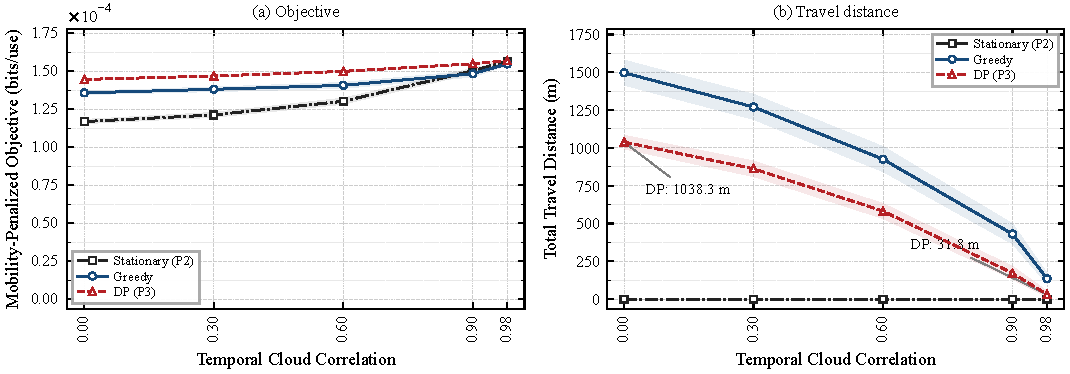
\includegraphics[width=\textwidth]{figures/fig3_temporal_correlation.pdf}
\caption{Latent temporal correlation at $p=0.4$, $\ell=250$ m, and
$\lambda_{\rm ref}$: (a) mean objective; (b) total travel distance.
Methods share 100 mission IDs; bands are pointwise 95\% whole-mission
bootstrap intervals. Latent $\rho$ differs from binary cloud correlation.}
\label{fig:temporal}
\end{figure*}

Fig.~\ref{fig:temporal} shows persistent favorable locations making offline
stationary selection competitive. As $\rho$ increases from
0 to 0.98, mean DP distance falls from 1038.25 to 31.84 m, while its mean
objective gain over P2 falls from 23.712\% to 0.155\%. This sampled trend
is not a correlation monotonicity theorem or an online result. Enlarging
nested position sets, however, cannot lower optimal P2/DP $U$: increasing
$J$ from 10 to 100 improves mean DP $U$ by 11.409\%.

At the default configuration and $\lambda_{\rm ref}$, DP improves mean
usable rate by 4.16\% over P2 and 2.70\% over Greedy, and mean objective
by 3.07\% and 4.42\%, respectively. Relative to zero-penalty DP, the
representative penalty reduces mean travel by 88.370\% with only a 0.515\%
decrease in mean usable rate. All locations select the same
MB source $(\nu,V_A)=(0.125,8)$ at the catalog boundary; these gains
do not isolate shaping gain. Rates retain the security limitations of
Section~\ref{sec:security}; finite-key, tracking, and nonideal-detector
effects~\cite{usenko2016} are excluded.

\section{Conclusion}
\label{sec:conclusion}
Finite-catalog MB source selection and cloud-aware positioning were
compared through Stationary, current-slot Greedy, and offline DP.
DP optimizes the finite-grid penalized objective, with observed blockage
avoidance and a favorable rate--distance tradeoff. Findings remain
conditional on synthetic clouds, offline information, and a distance-cost
surrogate. The two-dimensional MI and homodyne-conditioned Holevo
expressions are not measurement-consistent; a consistent security model
is required before these numerical rates can represent secure keys.

